% This file was created with tikzplotlib v0.10.1.
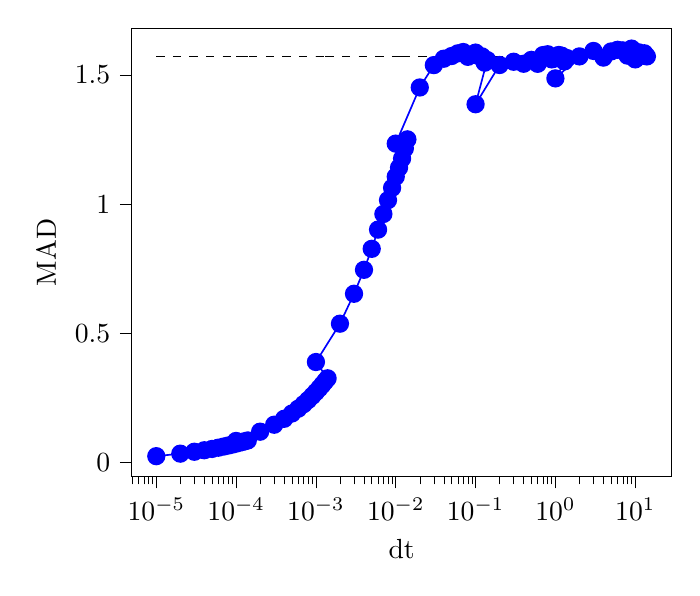
\begin{tikzpicture}

\definecolor{darkgray176}{RGB}{176,176,176}

\begin{axis}[
log basis x={10},
tick align=outside,
tick pos=left,
x grid style={darkgray176},
xlabel={dt},
xmin=4.92825984567174e-06, xmax=28.4075930214913,
xmode=log,
xtick style={color=black},
y grid style={darkgray176},
ylabel={MAD},
ymin=-0.0545205268080749, ymax=1.6808721165561,
ytick style={color=black}
]
\addplot [semithick, blue, mark=*, mark size=3, mark options={solid}]
table {%
1e-05 0.024360956981206
2e-05 0.0340582888051179
3e-05 0.0414777370123908
4e-05 0.0473391603613755
5e-05 0.0523460730306238
6e-05 0.0572038420872201
7e-05 0.0616172820275917
8e-05 0.0655831239703525
9e-05 0.0693904206547642
0.0001 0.0730602173513499
0.00011 0.0764593999663256
0.00012 0.0794074639742811
0.00013 0.0824461081310299
0.00014 0.0852260532823774
0.0001 0.0832831703261786
0.0002 0.119097877231027
0.0003 0.146008904290512
0.0004 0.168975495702742
0.0005 0.189511301079805
0.0006 0.208050658077013
0.0007 0.225439099084046
0.0008 0.241790929826209
0.0009 0.257541937784729
0.001 0.272588072531558
0.0011 0.286812639068708
0.0012 0.300413076356347
0.0013 0.313693941321929
0.0014 0.32571366364605
0.001 0.388806117390228
0.002 0.537145182434486
0.003 0.652925747249828
0.004 0.745717231989156
0.005 0.826920353306518
0.006 0.901250268231369
0.007 0.961734060125644
0.008 1.0153981590715
0.009 1.06291137221469
0.01 1.10624563535136
0.011 1.14109393018886
0.012 1.17657402491499
0.013 1.21540366709372
0.014 1.25072489449146
0.01 1.2342110873896
0.02 1.45159184849532
0.03 1.53808275914435
0.04 1.56290539776773
0.05 1.57321300381023
0.06 1.58364940726792
0.07 1.58878847825334
0.08 1.57013496792237
0.09 1.5773034805803
0.1 1.58646722155919
0.11 1.57299259477828
0.12 1.5719260417907
0.13 1.54737813708765
0.14 1.55758186740975
0.1 1.38663019539909
0.2 1.53846283208252
0.3 1.55107166824193
0.4 1.54329388673366
0.5 1.55835382804587
0.6 1.54315953258854
0.7 1.57703743891688
0.8 1.58017244440707
0.9 1.56025491148864
1 1.56385461581189
1.1 1.57733400134907
1.2 1.57453490254048
1.3 1.5524346785118
1.4 1.56520508286773
1 1.48671497306753
2 1.57176334586573
3 1.59290151371751
4 1.56713453617015
5 1.59107394835471
6 1.59736127456851
7 1.59514296000141
8 1.57480046677423
9 1.60199063276682
10 1.56031536224194
11 1.58767527922227
12 1.57479075224436
13 1.58382519863033
14 1.57170911217602
};
\addplot [semithick, black, dashed]
table {%
1e-05 1.5707963267949
2e-05 1.5707963267949
3e-05 1.5707963267949
4e-05 1.5707963267949
5e-05 1.5707963267949
6e-05 1.5707963267949
7e-05 1.5707963267949
8e-05 1.5707963267949
9e-05 1.5707963267949
0.0001 1.5707963267949
0.00011 1.5707963267949
0.00012 1.5707963267949
0.00013 1.5707963267949
0.00014 1.5707963267949
0.0001 1.5707963267949
0.0002 1.5707963267949
0.0003 1.5707963267949
0.0004 1.5707963267949
0.0005 1.5707963267949
0.0006 1.5707963267949
0.0007 1.5707963267949
0.0008 1.5707963267949
0.0009 1.5707963267949
0.001 1.5707963267949
0.0011 1.5707963267949
0.0012 1.5707963267949
0.0013 1.5707963267949
0.0014 1.5707963267949
0.001 1.5707963267949
0.002 1.5707963267949
0.003 1.5707963267949
0.004 1.5707963267949
0.005 1.5707963267949
0.006 1.5707963267949
0.007 1.5707963267949
0.008 1.5707963267949
0.009 1.5707963267949
0.01 1.5707963267949
0.011 1.5707963267949
0.012 1.5707963267949
0.013 1.5707963267949
0.014 1.5707963267949
0.01 1.5707963267949
0.02 1.5707963267949
0.03 1.5707963267949
0.04 1.5707963267949
0.05 1.5707963267949
0.06 1.5707963267949
0.07 1.5707963267949
0.08 1.5707963267949
0.09 1.5707963267949
0.1 1.5707963267949
0.11 1.5707963267949
0.12 1.5707963267949
0.13 1.5707963267949
0.14 1.5707963267949
0.1 1.5707963267949
0.2 1.5707963267949
0.3 1.5707963267949
0.4 1.5707963267949
0.5 1.5707963267949
0.6 1.5707963267949
0.7 1.5707963267949
0.8 1.5707963267949
0.9 1.5707963267949
1 1.5707963267949
1.1 1.5707963267949
1.2 1.5707963267949
1.3 1.5707963267949
1.4 1.5707963267949
1 1.5707963267949
2 1.5707963267949
3 1.5707963267949
4 1.5707963267949
5 1.5707963267949
6 1.5707963267949
7 1.5707963267949
8 1.5707963267949
9 1.5707963267949
10 1.5707963267949
11 1.5707963267949
12 1.5707963267949
13 1.5707963267949
14 1.5707963267949
};
\end{axis}

\end{tikzpicture}
